% !TEX program = xelatex

% 论文默认为双面模式,需单面模式请将第一行换为如下所示:
\documentclass[oneside]{zjucsmaster}

\begin{document}
\zjutitle{XXXXXXXX}{XXX的论文}
         {XXXXXXXX}{XXXXXXXX}

\zjuauthor{}{}
\zjuadvisor{}{}
\zjumajor{计算机科学与技术}{Computer Science and Technology}
\zjucollege{计算机科学与技术学院}{Computer Science and Technology}
\zjudate{2019年12月15日}{December 15, 2019}

{
    \pagestyle{empty} % remove header horizon line
    \begin{center}

{
    分类号: ~\zjuunderline{90pt}{}\hfill
    单位代码:~\zjuunderline{60pt}{10035}\\
    \vspace{3pt}
    密\quad 级:~\zjuunderline{90pt}{}\hfill
    学\quad\quad 号:~\zjuunderline{60pt}{}\\
}
    
{
    \vspace{10mm}
    
\includegraphics[width=7.78cm]{zjuname}\\
    \vspace{10mm}
    \yihao 硕~~~士~~~学~~~位~~~论~~~文 \\
    \vspace{10mm}
    
\includegraphics[width=3cm]{zjulogo}
}

{
    \vspace{10mm}
    \xiaoer
    {
        % \bfseries
        论文题目~ \underline{\makebox[10cm]{\zjutitlec}} \\
        \vspace{0.5cm}
        \hspace{4.6em} \underline{\makebox[10cm]{\zjutitlecl}}
    }

    \newlength{\titlelength}
    \setlength{\titlelength}{5.8cm}
    \vspace{2.22cm}
    \linespread{2.2} % 行间距,必须在字号之前设置
    \sihao
    作者姓名   ~ \underline{\makebox[\titlelength]{\zjuauthornamec}} \\
    指导教师   ~ \underline{\makebox[\titlelength]{\zjuadvisorc}} \\
    学科(专业) ~ \underline{\makebox[\titlelength - 1.3em]{\zjumajorc}} \\
    所在学院   ~ \underline{\makebox[\titlelength]{\zjucollegec}} \\
    提交日期   ~ \underline{\makebox[\titlelength]{\zjudatec}} \\
}

\end{center}

    \cleardoublepage
    \begin{center}
{
    \linespread{1}
    \erhao
    A Dissertation Submitted to Zhejiang\\
    University for the Degree of\\
    \vspace{0.3em} % Because the first line has extra line space.
    Master of Engineering\\
}

\vspace{0.95cm}

\includegraphics[width=3.0cm]{img/zjulogo}

{
    \vspace{3.15cm}
    \xiaoer
    TITLE: ~       \underline{\makebox[21em]{\zjutitlee}} \\
    \vspace{0.5cm}
    \hspace{4.0em} \underline{\makebox[21em]{\zjutitleel}}
}

\vspace{1.1em}

{
    \linespread{2}
    \begin{center}
        \sanhao
        \newlength{\majorlength}
        \setlength{\majorlength}{16em}
        \begin{tabular}{l l}
            Author: & \underline{\makebox[\majorlength]{\zjuauthornamee}} \\
            Supervisor: & \underline{\makebox[\majorlength]{\zjuadvisore}} \\
            Subject: & \underline{\makebox[\majorlength]{\zjumajore}} \\
            College: & \underline{\makebox[\majorlength]{\zjucollegee}} \\
            Submitted Date: & \underline{\makebox[\majorlength]{\zjudatee}} \\
        \end{tabular}
      \end{center}
}
\end{center}

    \cleardoublepage
    {
  \vspace*{0.6em}% * is for no discarding.
  {
    \centering
    \xiaoer
    浙江大学研究生学位论文独创性声明 \par
  }

  \vspace{3.1em}
  {
    \setlength{\parindent}{2em}
    \linespread{1.6}
    \xiaosi
    本人声明所呈交的学位论文是本人在导师指导下进行的研究工作及取得的研究成果。除了文中特别加以标注和致谢的地方外,论文中不包含其他人已经发表或撰写过的研究成果,也不包含为获得 \underline{\kaiti\sihao\bfseries \makebox[5em]{浙江大学}} 或其他教育机构的学位或证书而使用过的材料。与我一同工作的同志对本研究所做的任何贡献均已在文中作了明确的说明并表示谢意。 \par
  }

  \vspace{2.9em}
  {
    \xiaosi
    \begin{tabular}{@{} p{0.5\linewidth} p{0.5\linewidth} @{}}
    学位论文作者签名: & 日期: \hspace{4em} 年 \hspace{2em} 月 \hspace{2em} 日 \\
    \end{tabular} \par
  }

  \vspace{4.85em}
  {
    \centering
    \xiaoer
    学位论文版权使用授权书 \par
  }

  \vspace{2.2em}
  {
    \setlength{\parindent}{2em}
    \linespread{1.6}
    \xiaosi
    本文作者完全了解 \underline{\kaiti\sihao\bfseries \makebox[5em]{浙江大学}} 有权保留并向国家有关部门或机构送交本文的复印件和磁盘,允许本文被查阅和借阅。本人授权 \underline{\kaiti\sihao\bfseries \makebox[5em]{浙江大学}} 可以将学位论文的全部或部分内容编入有关数据库进行检索和传播,可以采用影印、缩印或扫描等复制手段保存、汇编学位论文。

    (保密的毕业论文(设计)在解密后适用本授权书) \par
  }

  \vspace{2.9em}

  {
    \xiaosi
    \begin{tabular}{@{} p{0.5\linewidth} p{0.5\linewidth} @{}}%@{} define space length
    学位论文作者签名: & 导师签名: \\
     & \\
     & \\
    日期: \hspace{4em} 年 \hspace{2em} 月 \hspace{2em} 日 & 日期: \hspace{4em} 年 \hspace{2em} 月 \hspace{2em} 日 \\
    \end{tabular} \par
  }
}

    \cleardoublepage
}

\newgeometry{top=37mm,bottom=37mm,left=31mm,right=31mm}

{
    \frontmatter  % remove "chapter 1" in section title, defined in book-like classes
    \makeatletter % fix catcode of '@', so that header works
      \let\ps@plain\ps@frontmatter
    \makeatother

    % todo: style of multi-page abstract is wrong
    \chapter{摘要}

这是摘要。目前多页摘要页眉会有问题。

\vspace{1em}
\setlength{\parindent}{0em}
\textbf{关键词}:~ todo~ todo~ todo

    \chapter{Abstract}

Todo...

\vspace{1em}
\setlength{\parindent}{0em}
\textbf{Keywords}:~ Quadrilateral Mesh, Mesh Quality, Geodesic Distance, Parameterization, Post-processing


    \pagestyle{frontmatter} % style for multi-page toc

    \tableofcontents
    \cleardoublepage

    {
      \let\oldnumberline\numberline
      \renewcommand{\numberline}{\figurename~\oldnumberline}
      \listoffigures
      \cleardoublepage
    }

    {
      \let\oldnumberline\numberline
      \renewcommand{\numberline}{\tablename~\oldnumberline}
      \listoftables
      \cleardoublepage
    }
}

{
    \mainmatter % restart counter
    \makeatletter % first page header and footer
      \let\ps@plain\ps@mainmatter
    \makeatother
    \pagestyle{mainmatter}

    \chapter{绪论}
\section{课题背景}

如图\ref{fig:aabb}所示,世界是复杂的,英文论文\cite{fang2018quadrangulation},中文论文\cite{sibianxingwanggezhiliang}。

\begin{figure}[h]
    \centering
    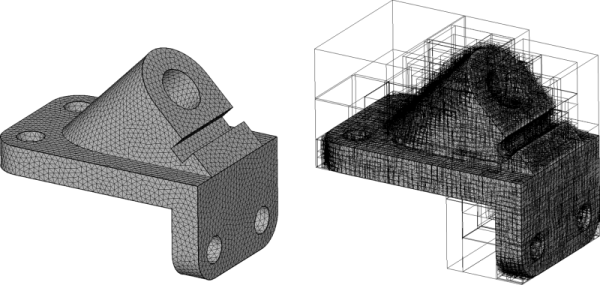
\includegraphics[width=5cm]{aabb}
    \caption[示意图]{示意图图图图图图图图图图图图图图图}
    \label{fig:aabb}
\end{figure}

\subsection{二级标题}

\subsubsection{三级标题}

测试表格\ref{tb:test}。

\begin{table}[h]
    \centering
    \begin{tabular}{|l|l|}
        \hline
        a & b \\ \hline
        c & d \\ \hline
    \end{tabular}
    \caption[测试表格]{测试表格格格格格格格格格格格格格}
    \label{tb:test}
\end{table}

引用结果章节\ref{chap:result}。

    \cleardoublepage

    \chapter{实验结果}
\label{chap:result}


    \cleardoublepage
}

{
    \backmatter
    \makeatletter
      \let\ps@plain\ps@backmatter
    \makeatother
    \pagestyle{backmatter}

    \bibliography{data/reference}
    % 将参考文献添加到目录
    \addcontentsline{toc}{chapter}{\bibname}
    \cleardoublepage

    \chapter{攻读硕士学位期间主要的研究成果}


    \cleardoublepage
    \chapter{致谢}

我真诚地感谢老师和同学们的帮助。

    \cleardoublepage
}

\end{document}
